\documentclass{article}
\usepackage{graphicx}
\usepackage[margin=0.75in]{geometry}
\begin{document}
\title{BIOS 611 Project-1}
\author{A. Virkud \\ e-mail: avirkud@unc.edu}
\date{October 19, 2020}
\maketitle
\section{Introduction and Data Source}
This report described the examination of heart failure patients in the MIMIC-IV dataset. The MIMIC-IV dataset has served as an important date for multiple machine learning efforts in the field of health care.\\
\\
MIMIC-IV is a retrospectively collected datasource containing electronic health record (EHR) data from Beth Israel Deaconess Medical Center (BIDMC). These data are deidentified records with information on patient experiences in the ICU. This analysis will use a subset of this data restricted to patients who are admitted with a heart failure diagnosis. MIMIC-IV is an excellent data source to examine the risk factors predicting heart failure since physicians have more and more been using and relying on their respective EHR systems to document patient diagnostics and histories. Additionally, this data system has access to all the lab results and procedures that patients received during their hospitalization.\\
\\
A relevant quote from the MIMIC-IV website: "In recent years there has been a concerted move towards the adoption of digital health record systems in hospitals. In the US, nearly 96\% of hospitals had a digital electronic health record (EHR) in 2015. Retrospectively collected medical data has increasingly been used for epidemiology and predictive modeling. The latter is in part due to the effectiveness of modeling approaches on large datasets"
\section{Objective}
The goal of this project is to characterize the features of heart failure patients in this the MIMIC-IV dataset. One of the original goals of this project was to predict mortality. In exploring the data, it was identified that many patients are missing death information since death certificates are no longer linked to this data source. 
\section{Methods}
Data were formatted and merged in Datasetup.R. Race/ethnicity, language, insurance, and marital status details were obtained from their most recent hospitalization. 
\section{Results}
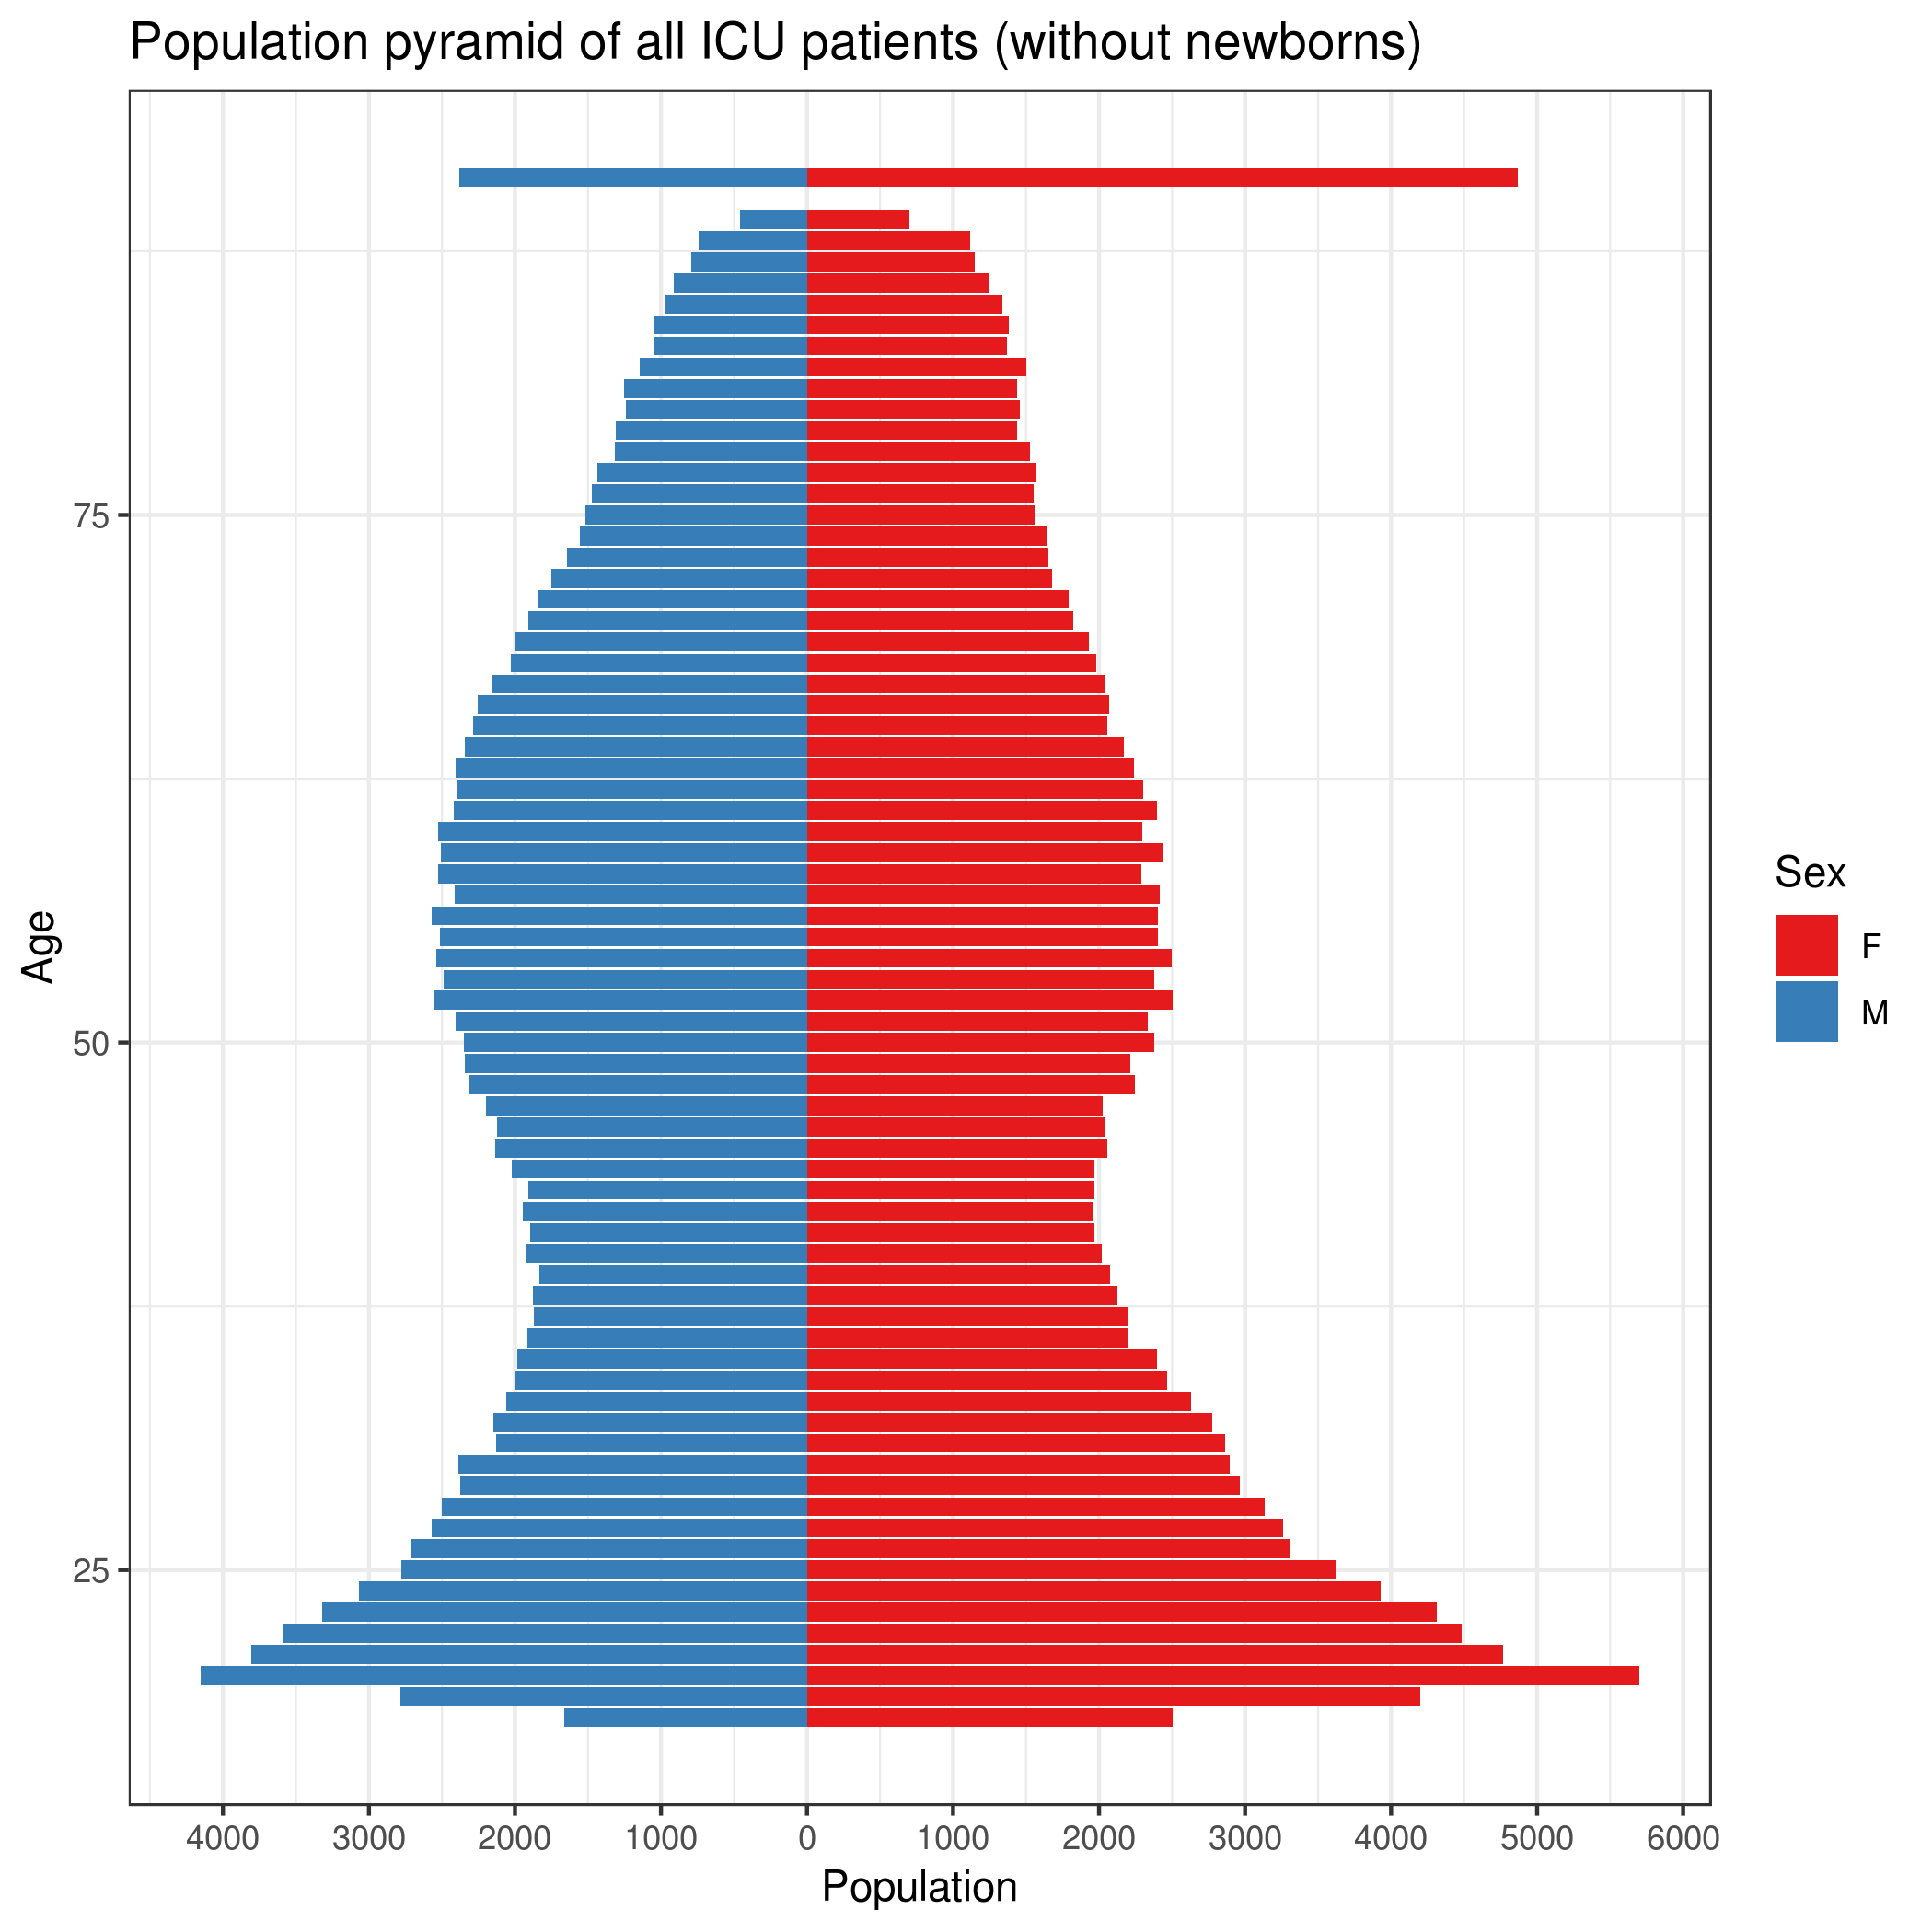
\includegraphics[width=0.5\textwidth]{figures/all_age_sex.png}\\
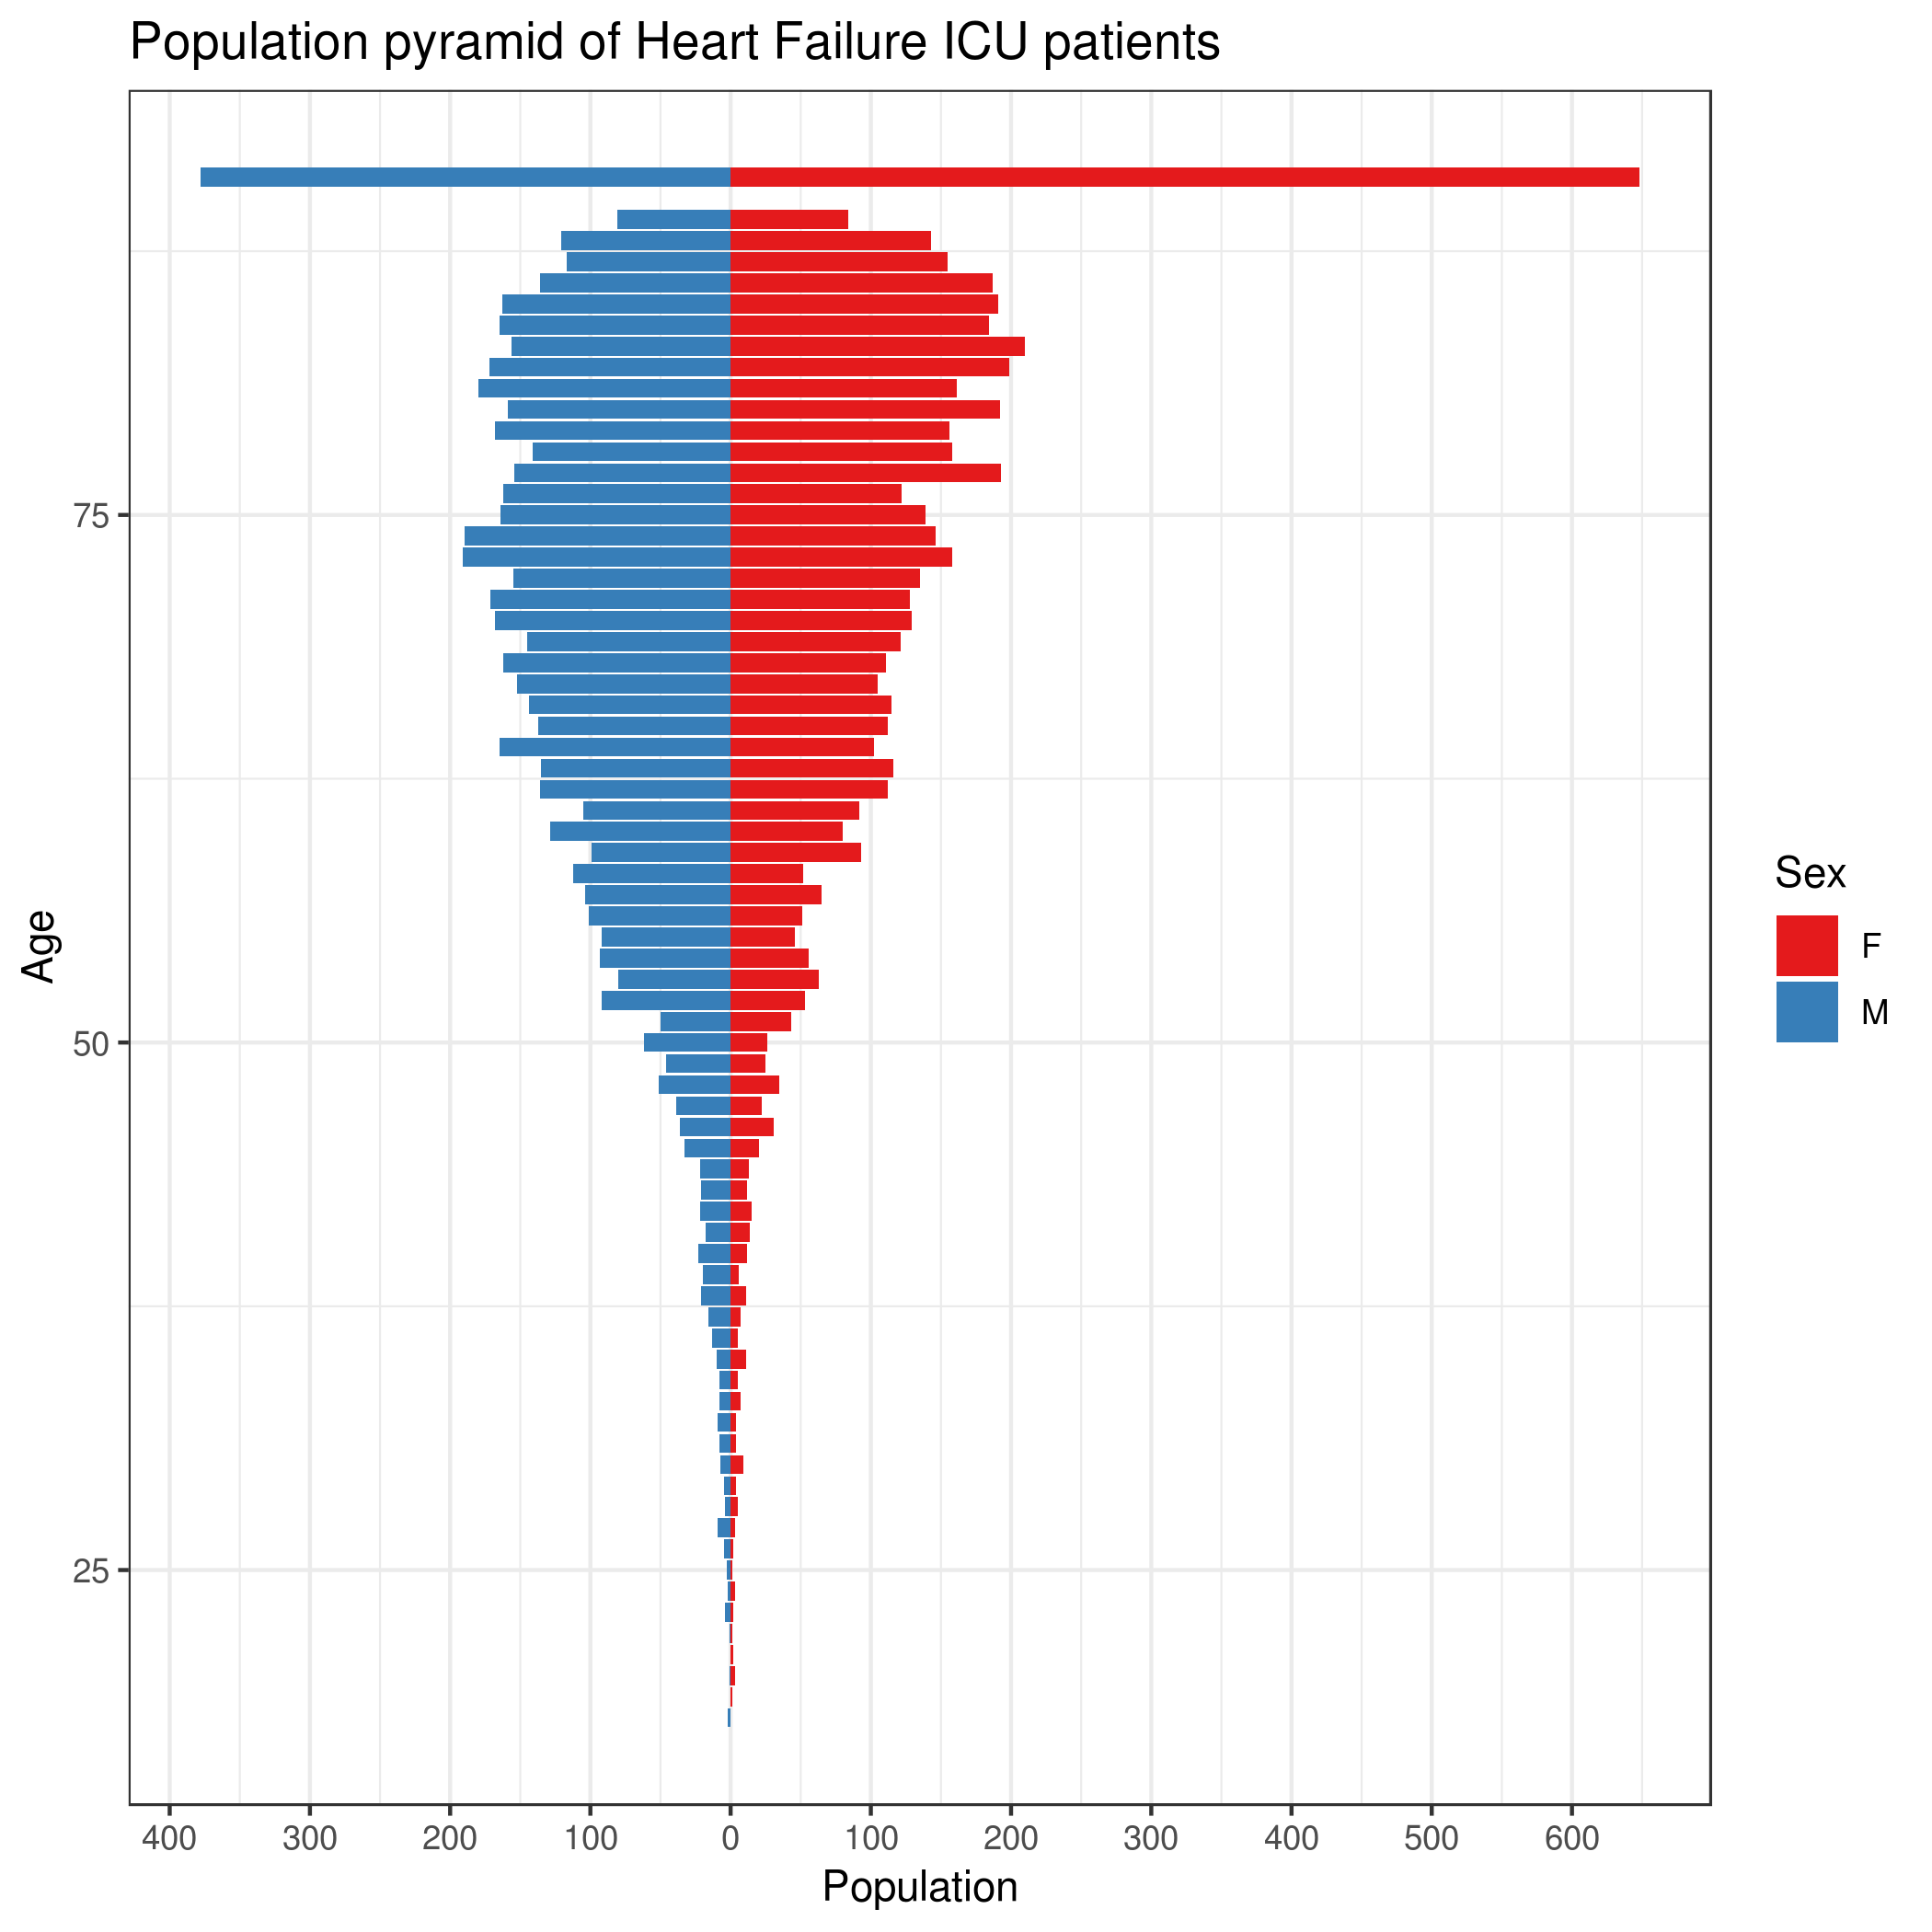
\includegraphics[width=0.5\textwidth]{figures/hf_age_sex.png}\\
\includegraphics[width=0.5\textwidth]{figures/all_age_sex_new.png}\\
Many of the patients admitted to the ICU are newborns.\\
Most heart failure patients in MIMIC-IV were over the age of 50. Interestingly, there were no patients aged 90 in this dataset, which suggests some error in data processing, since it is unlikely an ICU did not observe any 90-year-olds. If this missing data is genuine, it may indicate this data is not representative of all ICU settings. Additionally, the vast majority of individuals were 91, which possible represents a categorization of all individuals over the age of 90.\\
Among all heart failure patients 52.2\% were male and the majority were white (72.3\%), married, and spoke English. The most common medications were sodium chloride flushes, acetominophen, and furosemide, a loop diuretic. Only 2.8\% (343 individuals out of 11,981) of the heart failure population died in the hospital, which was lower than I originally expected. Because in-hospital death is rare in this population, predictive modelling would produce challenges in generalizability of results and interpretation.\\
\includegraphics[width=0.5\textwidth]{figures/eth_sex.png}\\
AI/AA stands for American Indian/Alaskan American (which are inappropriately lumped together). HL stands for Hispanic/Latino (which are not mutually exclusive to other racial identities categorized here. Unable stands for unable to obtain. Other, Unable to obtain, and Unknown represent roughly 8.4\% of the population. The average age was not substantially different across ethnicity groups.\\
\includegraphics[width=0.5\textwidth]{figures/Log_ROC.png}\\
The above figure is produced by applying logistic regression to classify deaths using age, ethnicity, marital status, language, and binary medication variables (for Loop Diuretics, Aspirin, Nitroglycerin, Warfarin, Statins, and Insulin) to predict death. This classifier does not perform well. I theorize this is due to the limited number of deaths in the dataset, and that logistic regression is not a sufficiently robust tool to classify the rare outcomes in this setting.\\

\section{Limitations and Further Analysis}
There are many more analyses that can be done with this data source. This fact is emphasized by how many machine learning papers in the area of health care research utilize MIMIC-IV. For the purposes of this course, several advanced analyses are not depicted in this report due to the size of the datasets required. Additional analyses would have included more variables from prescriptions and chart events to advance the predictive power of the optimal prediction method. Specifically, a binary indicator variable could have been included for prediction of mortality comparing results using logistic regression, LASSO, and Elastic Net. Additionally, propensity scores using demographic variables to evaluate the propensity for the most common medications could have been identified using logistic regression or random forest. 
\end{document}